\documentclass[12pt,a4paper]{article}
\usepackage[utf8]{inputenc}
\usepackage[english]{babel}
\usepackage{amsmath}
\usepackage{amsfonts}
\usepackage{amssymb}
\usepackage[left=2cm,right=2cm,top=2cm,bottom=2cm]{geometry}
\usepackage[x11names, rgb]{xcolor}
\usepackage{tikz}
\usetikzlibrary{trees,decorations,arrows,shapes,calc}

\author{Jiejia Xu}
\begin{document}

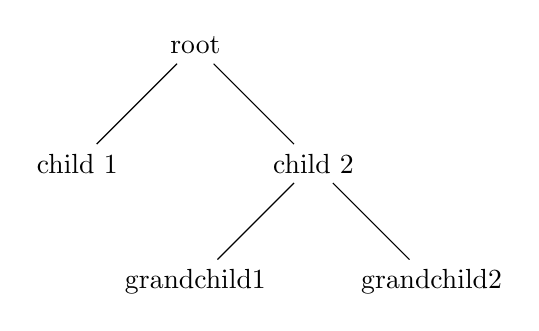
\begin{tikzpicture}
[sibling distance = 3cm]
\node(0){root}
	child{node(1){child 1}}
	child{node(2){child 2}
		child{node(3) {grandchild1}}
		child{node(4) {grandchild2}}	
	}
;
\end{tikzpicture}

\vspace{1cm}


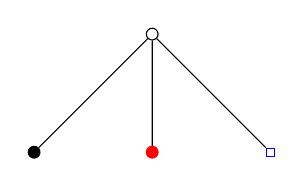
\begin{tikzpicture}
\tikzset{
	hollow node/.style = {circle, draw, inner sep = 1.5},
	solid node/.style = {circle, draw, inner sep = 1.5,fill = black},
	red node/.style = {circle, draw = red, inner sep = 1.5,fill = red},
	blue node/.style = {rectangle, draw = blue, inner sep = 1.5}
}

\node(0)[hollow node]{}
	child{node [solid node]{}}
	child{node [red node]{}}
	child{node [blue node]{}}
;
\end{tikzpicture}
\hspace{0.5cm}
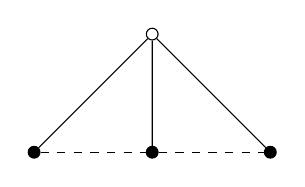
\begin{tikzpicture}
\tikzset{
	hollow node/.style = {circle, draw, inner sep = 1.5},
	solid node/.style = {circle, draw, inner sep = 1.5,fill = black},
}

\node(0)[hollow node]{}
	child{node [solid node]{}}
	child{node [solid node]{}}
	child{node [solid node]{}}
;

\draw [dashed] (0-1) to (0-2) to (0-3);

\end{tikzpicture}
\hspace{0.5cm}
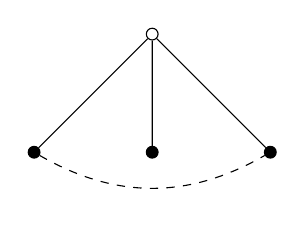
\begin{tikzpicture}
\tikzset{
	hollow node/.style = {circle, draw, inner sep = 1.5},
	solid node/.style = {circle, draw, inner sep = 1.5,fill = black},
}

\node(0)[hollow node]{}
	child{node [solid node]{}}
	child{node [solid node]{}}
	child{node [solid node]{}}
;

\draw [dashed, bend right] (0-1) to (0-3);

\end{tikzpicture}

\vspace{1cm}

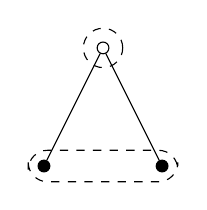
\begin{tikzpicture}
\tikzset{
	hollow node/.style = {circle, draw, inner sep = 1.5},
	solid node/.style = {circle, draw, inner sep = 1.5,fill = black},
}

\node(0)[hollow node]{}
	child{node [solid node]{}}
	child{node [solid node]{}}
;
\draw [dashed] (0) circle(0.25cm);
\draw [dashed, rounded corners = 7] ($(0-1)+(-0.2,-0.2)$) rectangle ($(0-2)+(0.2,0.2)$);

\end{tikzpicture}
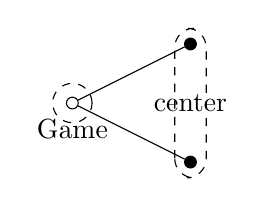
\begin{tikzpicture}
[grow = 0]
\tikzset{
	hollow node/.style = {circle, draw, inner sep = 1.5},
	solid node/.style = {circle, draw, inner sep = 1.5,fill = black},
}

\node(0)[hollow node, label = below:{Game}]{}
	child{node [solid node]{}}
	child{node [solid node]{}}
;
\draw [dashed] (0) circle(0.25cm);
\draw [dashed, rounded corners = 7] ($(0-1)+(-0.2,-0.2)$) rectangle ($(0-2)+(0.2,0.2)$);
\node at($(0-1)!.5!(0-2)$) {center};

\end{tikzpicture}

\vspace{1cm}

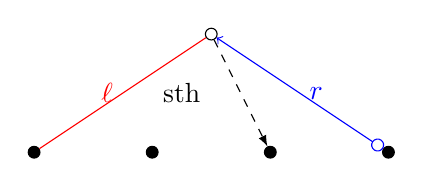
\begin{tikzpicture}
\tikzset{
	hollow node/.style = {circle, draw, inner sep = 1.5},
	solid node/.style = {circle, draw, inner sep = 1.5,fill = black},
}

\node(0)[hollow node]{}
	child{node [solid node]{} edge from parent [red] node [left]{$\ell$}}
	child{node [solid node]{} edge from parent [draw= none] node {sth}}
	child{node [solid node]{} edge from parent [->,>=latex,dashed]}
	child{node [solid node]{} edge from parent [<-o,blue]node[right]{$r$}}
;

\end{tikzpicture}


\vspace{1cm}

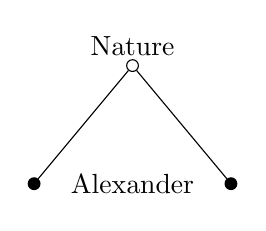
\begin{tikzpicture}
\tikzset{
	hollow node/.style = {circle, draw, inner sep = 1.5},
	solid node/.style = {circle, draw, inner sep = 1.5,fill = black},
}
\node(0)[hollow node]{}
[sibling distance=25mm]
child{node[solid node]{}}
child{node[solid node]{}}
;
\node[above]at(0){Nature};
\node at($(0-1)!.5!(0-2)$){Alexander};
\end{tikzpicture}
\hspace{0.5cm}
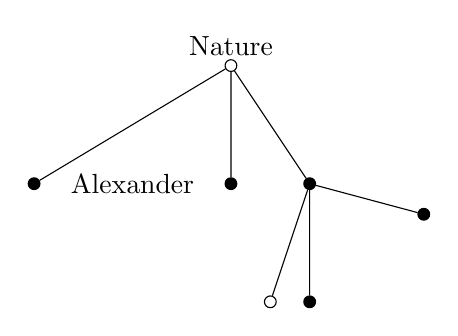
\begin{tikzpicture}
\tikzset{
	hollow node/.style = {circle, draw, inner sep = 1.5},
	solid node/.style = {circle, draw, inner sep = 1.5,fill = black},
	level 1/.style = {sibling distance=25mm},
	level 2/.style = {sibling distance=5mm}
}
\node(0)[hollow node]{}
child{node[solid node]{}}
child{node[solid node]{}}
child[sibling distance=10mm]{node[solid node]{}
		child{node[hollow node]{}}
		child{node[solid node]{}}
		child[grow = -15]{node[solid node]{}}
	}
;
\node[above]at(0){Nature};
\node at($(0-1)!.5!(0-2)$){Alexander};
\end{tikzpicture}

\vspace{1cm}
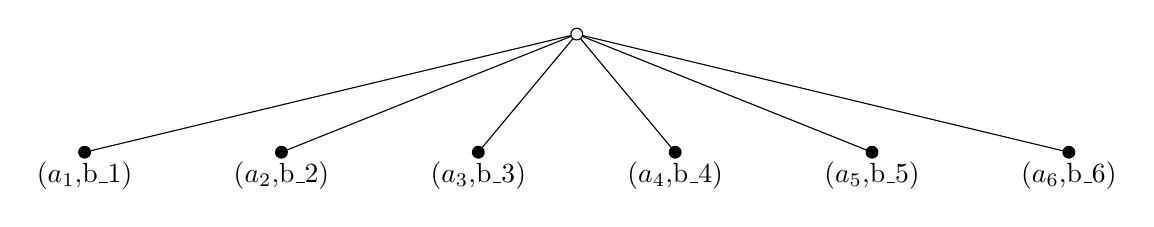
\begin{tikzpicture}
\tikzset{
	hollow node/.style = {circle, draw, inner sep = 1.5},
	solid node/.style = {circle, draw, inner sep = 1.5,fill = black},
	level 1/.style = {sibling distance=25mm},
}
\node(0)[hollow node]{}
child{node[solid node]{}}
child{node[solid node]{}}
child{node[solid node]{}}
child{node[solid node]{}}
child{node[solid node]{}}
child{node[solid node]{}}
;

\foreach \i in {1,...,6} \node [below] at (0-\i) {($a_\i$,b\_\i)};

\end{tikzpicture}


\vspace{1cm}
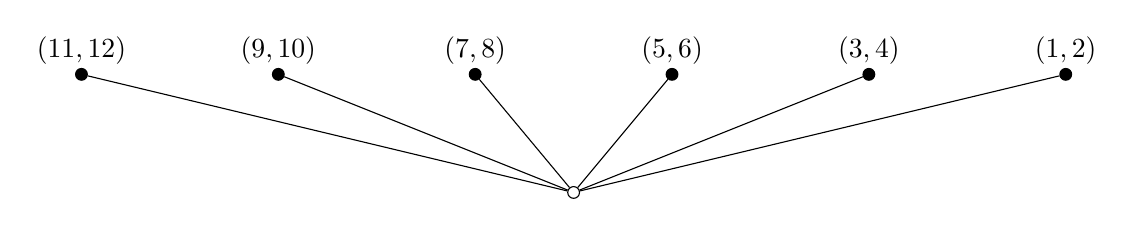
\begin{tikzpicture}
\tikzset{
	hollow node/.style = {circle, draw, inner sep = 1.5},
	solid node/.style = {circle, draw, inner sep = 1.5,fill = black},
	level 1/.style = {sibling distance=25mm},
}

\node(0)[hollow node]{}
[grow = 90]
child{node[solid node]{}}
child{node[solid node]{}}
child{node[solid node]{}}
child{node[solid node]{}}
child{node[solid node]{}}
child{node[solid node]{}}
;

\foreach \i in {1,...,6}
	\pgfmathsetmacro{\payoffa}{2*\i-1}
	\pgfmathsetmacro{\payoffb}{2*\i}
	\node[above]at (0-\i)
		{$(\pgfmathprintnumber{\payoffa},\pgfmathprintnumber{\payoffb})$};

\end{tikzpicture}



\end{document}